%
\begin{figure*}[ht]
\begin{center}
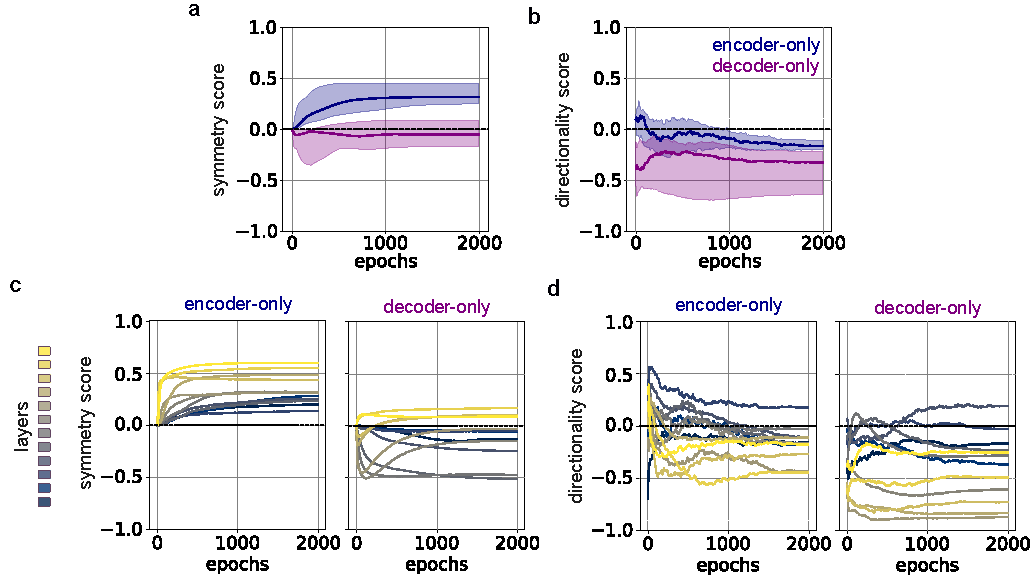
\includegraphics[width=1.\linewidth]{ICML2025/figures/figures-pdf/figure-training-layers.pdf}
\end{center}
%
\caption{
%
\textbf{a})
%
Evolution of symmetry score during training.
%
We train a Bert-base-uncased model with 12 layers on the Wikipedia dataset  \citep{wikidump} in encoder-only (blue) and decoder-only (purple) mode, see legend.
%
Shown are the median and the interquartile range.
%
Shown are the median and the interquartile range.
%
\textbf{b})
%
Same as in panel \textbf{a}
for the median directionality score.
%
\textbf{c})
%
Evolution of the median symmetry score across layers of the encoder-only (left) and decoder-only (right) models.
%
Each layer is color-coded as shown on the legend.
%
\textbf{d})
%
Same as panel $\textbf{c}$ for the median directionality score.
%
}
%
\label{fig-training-layers}
%
\end{figure*}